\section{Methodology}

%%%%%%%%%%%%%%%%%%%%%%%%%%%%%%%%%%%%%%%%%%%%%%%%%%%%%%%%%%%%%
% Mean Flow
%%%%%%%%%%%%%%%%%%%%%%%%%%%%%%%%%%%%%%%%%%%%%%%%%%%%%%%%%%%%%
\subsection{Mean Flow}

\begin{figure}[b]
  \centering
  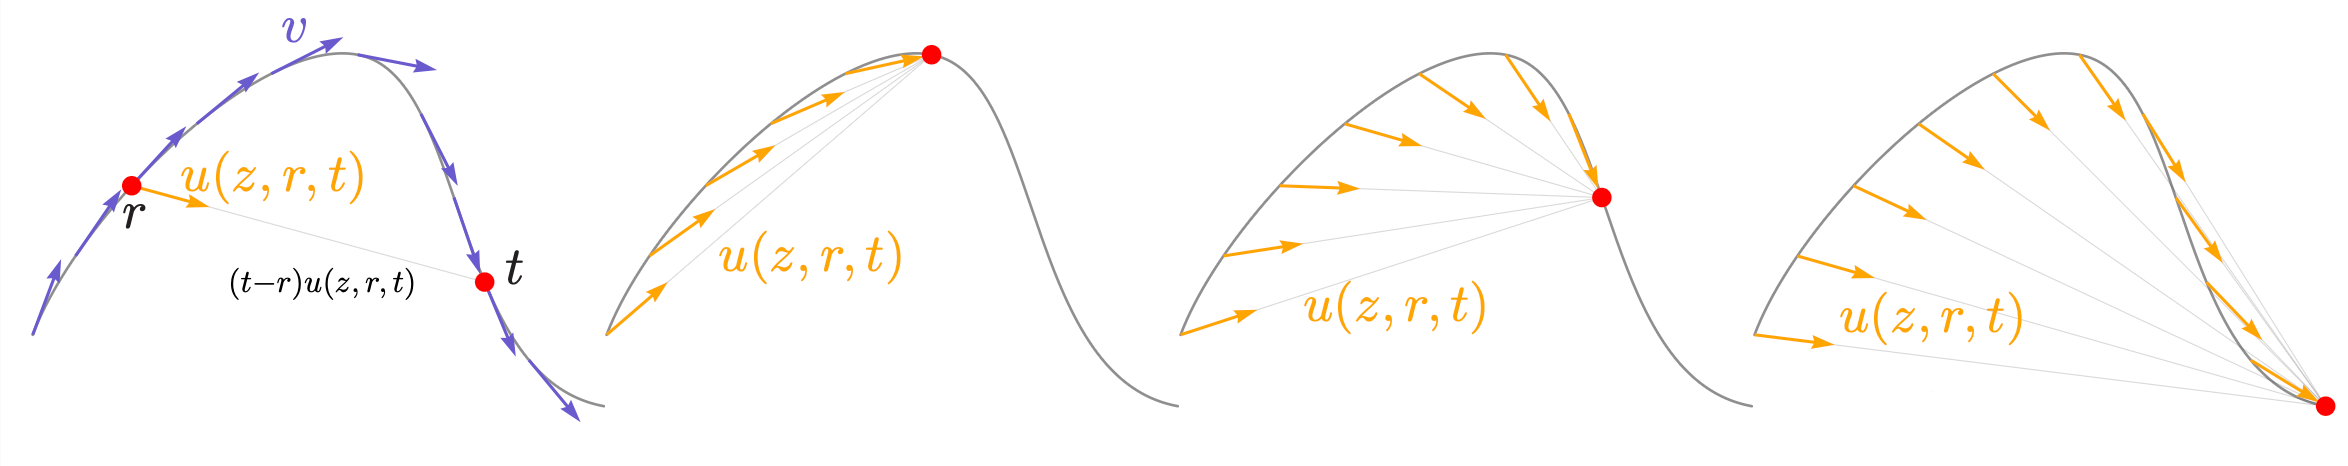
\includegraphics[width=\textwidth]{figures/meanflows.png}
  \caption{Illustration of the average velocity $u(z, r, t)$. Here, $z$ means the current location, i.e. $x_r$ in Equation~\eqref{average_velocity}. Leftmost: The instantaneous velocity $v(x_t, t)$. Right three subplots: The average velocity field at different time $t$. Figure revised from~\cite{meanflow}.}
  \vspace{-3em}
\end{figure}

Following~\cite{meanflow}, the instantaneous velocity field in Flow Matching can be replaced with an average velocity to enable one-step generation. Specifically, from time $r$ to time $t$, the average velocity is defined as:
%
\begin{equation}\label{average_velocity}
  u(x_r, r, t) \triangleq \frac{1}{t - r} \int^t_r v(x_\tau, \tau) \; d \tau.
\end{equation}
%
Rewrite Equation~\eqref{average_velocity} as $(t - r) u(x_r, r, t) = \int_r^t v(x_\tau, \tau) \, d \tau$, and differentiate both sides with respect to $r$:
%:
\begin{equation*}
  u(x_r, r, t) = v(x_r, t) + (t - r) \frac{d}{d r} u(x_r, r, t),
\end{equation*}
%
Applying the total derivative theorem, we obtain:
\begin{align}
  u(x_r, r, t) &= v(x_r, r) + (t - r) \left( \frac{\partial u}{\partial x_r} \frac{d x_r}{d r} + \frac{\partial u}{\partial t} \frac{d t}{d r} +  \frac{\partial u}{\partial r} \frac{d r}{d r} \right) \nonumber \\
  &= v(x_r, r) + (t - r) \left( \frac{\partial u}{\partial x_r} v(x_r, r) + \frac{\partial u}{\partial r}\right)
\end{align}
%
since $\dfrac{dt}{dr} = 0$ and $\dfrac{dx_r}{dr} = v(x_r, r)$.

Similiar to Flow Matching, we train a neural network $u^\theta(x_r, r, t)$ to approximate $u(x_r, r, t)$ with an MSE loss:
\begin{equation}
  \mathcal{L_\text{MF}} (\theta) = \mathbb{E}_{r, t, x_r \sim p_r} \left[ \left\| u^\theta(x_r, r, t) - \text{sg} \left[u^\text{tgt} (x_r, r, t)\right] \right\|_2^2 \right],
\end{equation}
%
where $\text{sg}\left[ \cdot \right]$ denotes the stop gradient operator and $u^\text{tgt}(x_r, r, t)$ is given by:
\begin{equation}\label{mf_basic_eq}
  u^\text{tgt} (x_r, r, t) =  v^\text{tgt}(x_r, r) + (t - r) \left( \frac{\partial u^\theta}{\partial x_r} v^\text{tgt}(x_r, r) + \frac{\partial u^\theta}{\partial r}\right).
\end{equation}
%
Here, the derivatives of $u$ are approximated by those of $u^\theta$, following~\cite{meanflow}.

Since the error term $u^\theta(x_r, r, t) - \text{sg} \left[u^\text{tgt} (x_r, r, t) \right]$ is a linear function of $v^\text{tgt}(x_r, r)$, and according to the result in Appendix~\ref{app:linear_func}, this allows $v^\text{tgt}(x_r, r)$ to be substituted with the conditional velocity $v(x_r, r \mid z)$:
%
\begin{align}
   \mathcal{L_\text{CMF}} (\theta) &= \mathbb{E}_{r, t, z \sim p_\text{target}, x_r \sim p_r(\cdot \mid z)} \left[ \left\| u^\theta(x_r, r, t) - \text{sg} \left[u^\text{cond} (x_r, r, t) \right] \right\|_2^2 \right] \\
   u^\text{cond} &=  v(x_r, r \mid z) + (t - r) \left( \frac{\partial u^\theta}{\partial x_r} v(x_r, r \mid z) + \frac{\partial u^\theta}{\partial r} \right)
\end{align}

This formulation allows MeanFlow to be trained similar to Flow Matching, while directly targeting on the average velocity field to enable the one-step generation. The derivative term $\dfrac{d u^\theta}{d r}$ is computed using the Jacobian-Vector-Product (JVP) operation, such as \texttt{torch.func.jvp} in PyTorch. Besides, classifier-free guidance (CFG) is also incoporated into the MeanFlow. According to~\cite{meanflow}, the CFG conditional MSE loss is defined as:
%
\begin{align}
  \mathcal{L_\text{CMF}^\text{cfg}} (\theta) &= \mathbb{E}_{r, t, x_r \sim p_r} \left[ \left\| u_\text{cfg}^\theta(x_r, r, t \mid c) - \text{sg} \left[u_\text{cfg}^\text{cond} (x_r, r, t \mid c)\right] \right\|_2^2 \right] \\
  u_\text{cfg}^\text{cond} (x_r, r, t \mid c) &= v_\text{cfg}(x_r, r \mid c, z) + (t - r) \left( \frac{\partial u^\theta}{\partial x_r} v_\text{cfg}(x_r, r \mid c, z) + \frac{\partial u^\theta}{\partial r} \right), \label{mf_cfg_tgt}
\end{align}
%
where the CFG-enhanced conditional velocity $v_\text{cfg} (x_r, r \mid c, z)$ is given by:
%
\begin{equation}\label{v_cond_cfg}
  v_\text{cfg} (x_r, r \mid c, z) = \omega v(x_r, r \mid z) + (1 - \omega) u_\text{cfg}^\theta (x_r, r, r)
\end{equation}
%
The details are provided in Appendix~\ref{app:cfg}.



%%%%%%%%%%%%%%%%%%%%%%%%%%%%%%%%%%%%%%%%%%%%%%%%%%%%%%%%%%%%%
% Change the Prior for Denoising
%%%%%%%%%%%%%%%%%%%%%%%%%%%%%%%%%%%%%%%%%%%%%%%%%%%%%%%%%%%%%
\subsection{Change the Prior for Denoising}

To serve the denoising purpose, we alter the $p_\text{prior}$ to be noisy images rather than simple distributions like the standard Gaussian. This modification enables the average velocity to directly model the transformation from noisy images to clean images.

%%%%%%%%%%%%%%%%%%%%%%%%%%%%%%%%%%%%%%%%%%%%%%%%%%%%%%%%%%%%%
% DiT Architecture
%%%%%%%%%%%%%%%%%%%%%%%%%%%%%%%%%%%%%%%%%%%%%%%%%%%%%%%%%%%%%
\subsection{DiT Architecture}\label{sec:dit}

\begin{figure}[h]
  \centering
  \begin{minipage}[t]{0.40\textwidth}
  \setstretch{1.3} % 设置这一段文字的局部行距为1.3倍
  We adopt the Diffusion Transformer (DiT) Architecture~\cite{dit} to parameterize the average velocity field. The input $x_t$ is divided into patches, linearly embedded, and encoded with sinusoid positional embeddings. Time informations (i.e., $r$ and $t$) are embedded by a lightweight MLP, while class labels are embedded with label embeddings. All embeddings are added to each transformer block through adaptive LayerNorm (adaLN), allowing time and conditional information to modulate both attention and feed-forward layers. The network backbone consists of stacked DiT blocks with multi-head self-attention and GELU-MLPs, followed by a final projection and unpatchify step.
  \end{minipage}
  %
  \begin{minipage}[t]{0.58\textwidth}
    \centering
    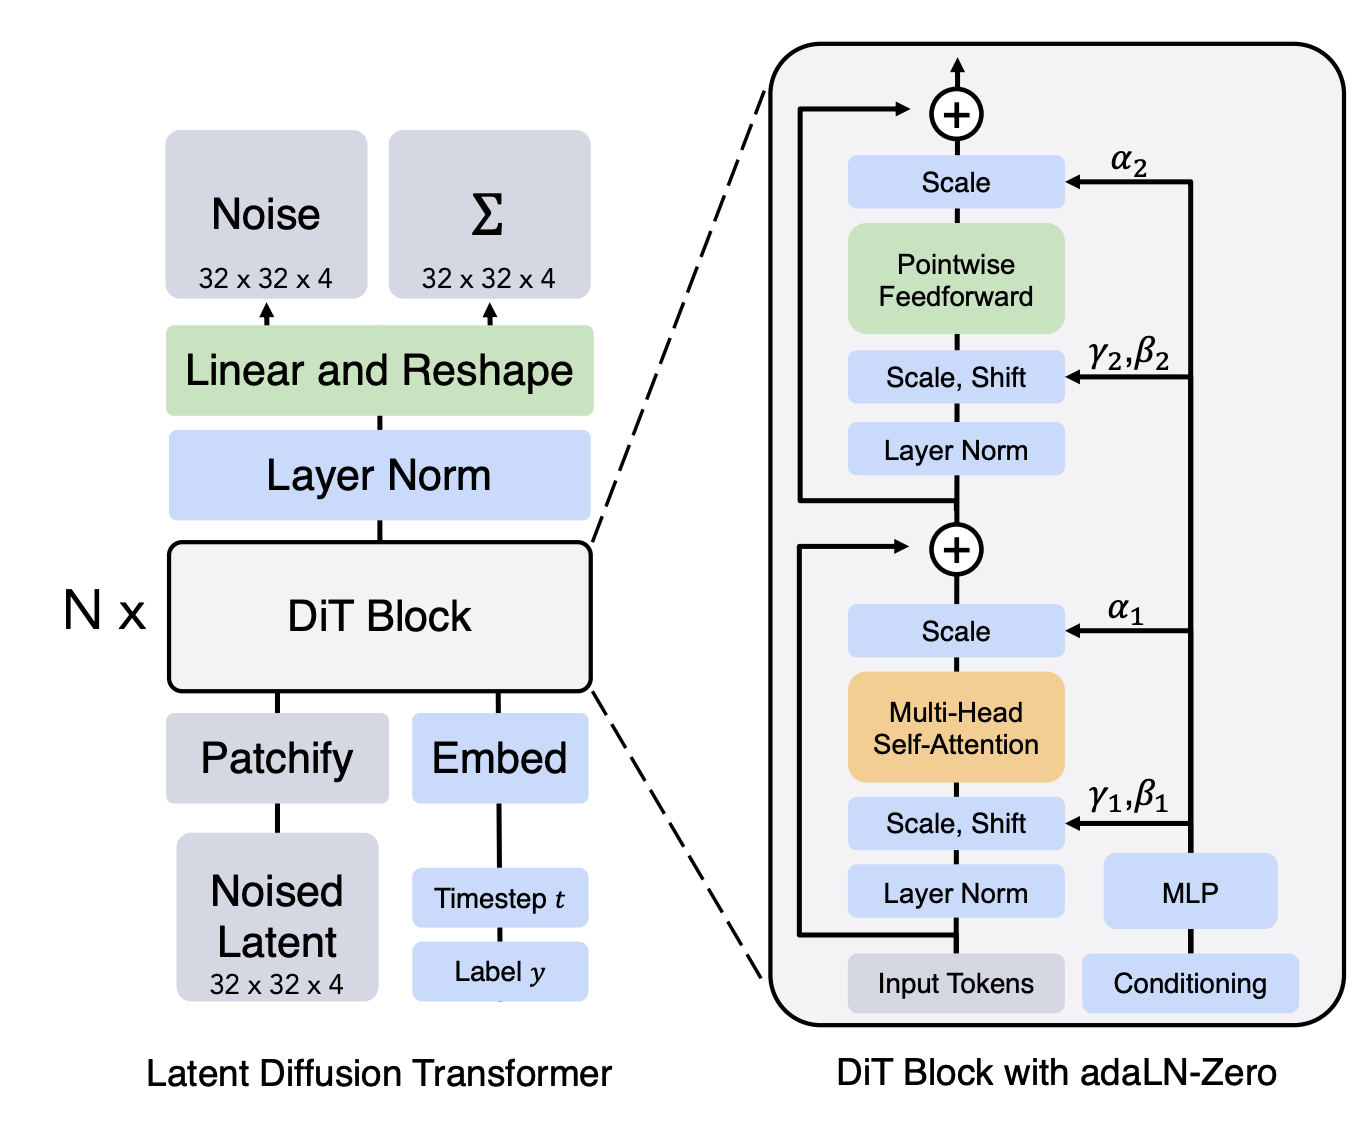
\includegraphics[width=\textwidth, valign=t]{figures/dit.png}
    \caption{Illustration of the DiT architecture. Figure from~\cite{dit}}
    \label{fig:DiT_arch}
  \end{minipage}
\end{figure}
